\section{RLPBWT con matching statistics}
Le precedenti versioni della \textit{RLPBWT}, come anticipato, hanno permesso di
poter ideare una variante \textit{run-length encoded} della \textit{PBWT}.
In realtà anche in questo caso c'è stata una fase transitoria di sviluppo,
avendo due varianti della struttura, che verranno introdotte a breve.\\
Il fine era quello di ottenere quanto visto per la \textbf{RLBWT} anche per la
variante posizionale, ovvero i concetti di:
\begin{itemize}
  \item \textit{matching statistics}
  \item \textit{threshold}
  \item \textit{LCE query}
\end{itemize}
A tal fine, come per la \textit{RLBWT}, si necessita di \textit{random access}
al testo. A causa di questo si sono avute due varianti in fase di sviluppo:
\begin{itemize}
  \item una prima, ancora in ottica di ``studio introduttivo'', dove il pannello
  viene memorizzato come \textit{vettore di bitvector classici}
  \item una seconda, definitiva, dove il pannello è memorizzato come
  \textit{SLP}, nelle modalità introdotte nella sottosezione \ref{subslp}
\end{itemize}
Questee versioni, a loro volta, hanno permesso, in primis, l'ideazione di un
algoritmo che sfruttasse l'idea delle threshold, come visto per la \textit{BWT}
classica con \textit{MONI} \cite{moni}, e poi, per quella basata
sull'\textit{SLP}, di uno basato sulle \textit{LCE query}, come per
\textit{PHONI} \cite{phoni}. Quest'ultima, con l'aggiunta della
\textit{struttura per la funzione $\varphi$}, sarà l'implementazione definitiva,
per questa tesi, della \textit{RLPBWT}.\\
Avendo in memoria il pannello si può quindi fare a meno dell'array \textit{LCP}
della colonna $k$-esima, avendo quindi che, per ogni colonna $k$, si ha in
memoria:
\begin{itemize}
  \item un booleano $start^k$ per specificare se la colonna presenta la prima
  run costruita su simboli $\sigma =0$
  \item un bitvector sparso $h_k$ per indicare l'inizio delle run
  \item il valore $c[k]$ per sapere quanti simboli $\sigma=0$ si hanno nella
  colonna 
  \item i valori $u_k$ e $v_k$ per il mapping
  \item i cosiddetti \textbf{prefix array samples}, ovvero i valori del
  \textbf{prefix array} di inizio e fine di ogni run. Si noti quindi che, anche
  in questo caso, si ha un'informazione in memoria proporzionale al numero di
  run $r$ 
\end{itemize}
In pratica si hanno in memoria le stesse informazioni della \textit{RLPBWT con
  bitvector} al più di $l_k$, ovvero l'\textit{array LCP} della colonna
$k$-esima, e dei \textit{prefix array samples}. 
\subsection{Matching statistics per la RLPBWT}
La definizione formale per il concetto di \textbf{matching statistics}, nonché
il calcolo dell'array stesso, vista per
la \textit{RLBWT} deve essere ovviamente riadattata allo studio di match tra un
aplotipo e un pannello di aplotipi.
\begin{definizione}
  Dato un pannello $X$, di dimensioni $M\times N$, con $M$ individui e $N$ siti,
  e un aplotipo esterno/pattern $z$, tale che $|z|=N$, si definisce matching
  statistics di $z$ su $X$ un array $MS$ di coppie $(row,len)$, di lunghezza
  $N$, tale che (avendo che $x_i$ indica l'$i$-esima riga del pannello $X$): 
  \begin{itemize}
    \item $x_{MS[i].row}[i-MS[i].len+1,i]=z[i-MS[i].len+1,i]$, ovvero si ha che
    l'aplotipo query ha un match, terminante in colonna $i$, con la riga
    $MS[i].row$  
    \item $z[i-MS[i].len,i]$ non è un suffisso terminante in colonna $i$ di un
    qualsiasi sottoinsieme di righe di $X$. In altri termini il match non deve
    essere ulteriormente estendibile a sinistra
  \end{itemize}
\end{definizione}
Inoltre, analogamente al caso della variante classica, si ha il seguente lemma.
\begin{lemma}
  Dato un pannello $X$, di dimensioni $M\times N$, con $M$ individui e $N$
  siti, un aplotipo esterno/pattern $z$, tale che $|z|=N$, e il corrispondente
  array di matching statistics $MS$ si ha che:
  \[z[i-l+1:i]\]
  è un \textbf{MEM} di lunghezza $l$ in con la riga $MS[i].row$ del pannello
  $X$ sse: 
  \[MS[i].len=l\land(i=N\lor MS[i].len\geq MS[i+1].len)\]
\end{lemma}
\textit{Si vedrà in sezione \ref{secphi} come calcolare, a partire da tali
  \emph{MEM}, tutte le righe del panello per le quali si ha lo stesso
  \textup{MEM}}.\\
Il calcolo dell'array $MS$ di $z$ rispetto al pannello $X$ si basa su due fasi:
\begin{enumerate}
  \item la fase di \textbf{extension}
  \item la fase di \textbf{bootstrap}
\end{enumerate}
Si assuma di avere due indici $i$ e $j$, $0\leq i\leq j\leq N$, tali per cui
$z[i,j]$ è un suffisso di uno tra $x_1[1,j]$, \ldots, $x_M[1,j]$. \\
La \textbf{fase di extension} estende il match di $z[i,j]$ a $z[i,j+1]$ sse:
\begin{itemize}
  \item $j<M$
  \item $z[i,j+1]$ è un suffisso di uno tra $x_1[1,j+1]$, $\ldots$, $x_M[1,j+1]$
\end{itemize}
D'altro canto la \textbf{fase di bootstrap} cerca il più piccolo indice $i'$,
avendo $i\leq i'\leq j$, tale per cui $z[i',j]$ è un suffisso di uno tra
$x_1[1,j+1]$, $\ldots$, $x_M[1,j+1]$.\\
Si ha quindi il computo di ogni valore $MS[i]$, $\forall i\in[0,N)$, dell'array
delle \textit{matching statistics}:
\begin{itemize}
  \item si assume inizialmente che $MS[0].len=0$
  \item si applica la \textit{fase di bootstrap} per cercare il minimo indice
  $i'$, avendo $i\leq i'$, tale che $z[i',i'+MS[i].len]$ è un suffisso di uno
  tra $x_1[1,i'+MS[i].len],$ \ldots$, x_M[1,i'+MS[i].len]$. Inoltre, per
  minimalità di $i'$ si ha che, $\forall i<j<i'$, $MS[j].len=MS[j-1].len+1$
  \item a questo punto si itera la \textit{fase di estensione} per trovare il
  più lungo prefisso $z[i',k]$ che è anche un suffisso di uno tra $x_1[1,k]$,
  $\ldots$, $x_M[1,k]$, avendo che $MS[i'].len=k-i'+1$
  \item avendo che $i'>i$ si può procedere induttivamente al calcolo dell'array
  $MS$ 
\end{itemize}
\textbf{PARTE PRESA DAL PAPER: RIVEDERE PROFONDAMENTE}.\\
In altri termini, più ``pratici'', il calcolo dell'array $MS$ avviene nel
seguente modo:
\begin{itemize}
  \item si parte da una riga arbitraria $i$ della prima colonna
  \item se $x_i[0]=z[0]$ si procede salvando $MS[0].row=i$
  \item qualora si abbia $x_i[0]\neq z[0]$ si seleziona o l'ultima riga della
  run precedente o la prima riga della run successiva a quella a cui appartiene
  la riga $i$. Tale riga, $j$, verrà salvata in $MS$, avendo $MS[0].row=j$
  \item a questo punto si effettua il mapping verso la colonna successiva, $k$,
  e, a seconda di avere un match con $z[k]$ si procede come nei casi visti sopra
\end{itemize}
Si noti che non si è parlato di come calcolare i vari $MS[i].len$, questo in
quanto si hanno due soluzioni (che verranno poi approfondite), che riprendono
appunto \textit{MONI} e \textit{PHONI} per la \textit{RLBWT};
\begin{enumerate}
  \item si possono usare le threshold per capire che nuova riga selezionare in
  caso di mismatch. In tal caso i vari $MS[i].len$ devono essere calcolati dopo
  il calcolo di $MS[i].row$ tramite \textit{random access} al panel
  \item si possono usare le \textit{LCE query} per capire che nuova riga
  selezionare in caso di mismatch e in tal caso il calcolo delle $MS[i].len$
  avviene in contemporanea 
\end{enumerate}
Prima di procedere con i dettagli dei due metodi è bene proporre un veloce
esempio di array $MS$.
\begin{esempio}
  Si riprenda nuovamente l'esempio \ref{es:algo5}, con un pannello e i match con
  la query $z$:
  \begin{figure}[H]
    \centering
    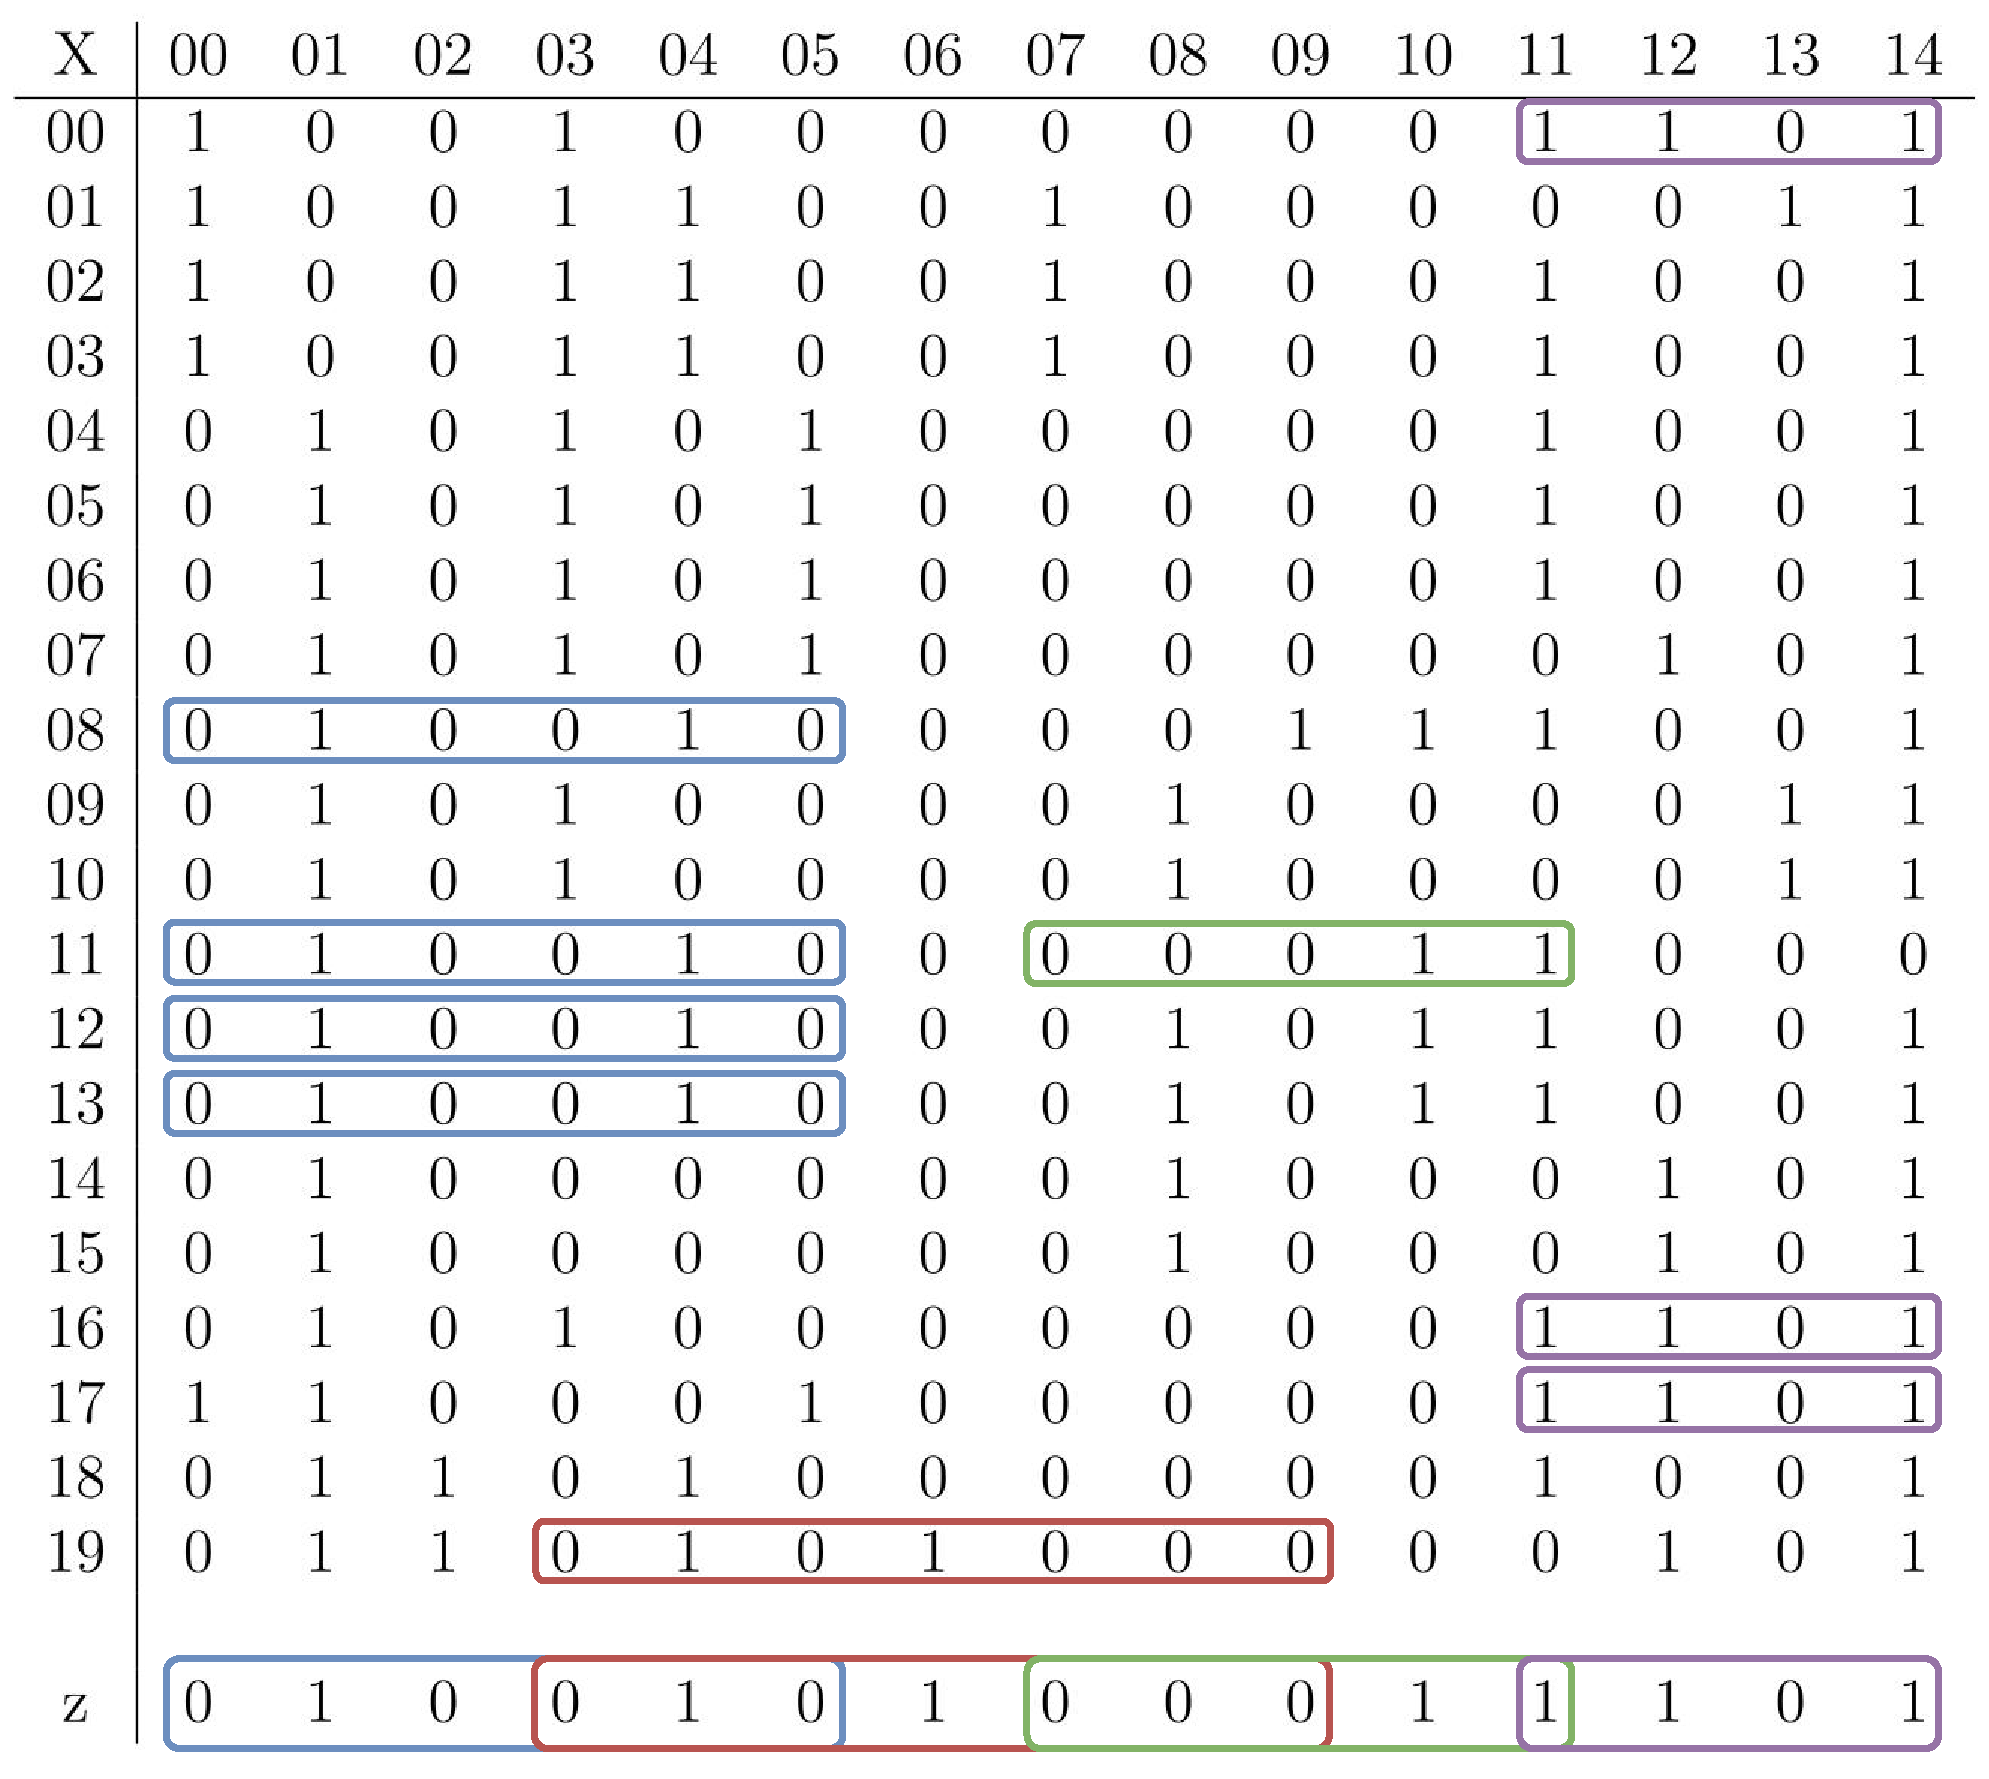
\includegraphics[scale = 0.365]{img/pbwtmatch.pdf}
  \end{figure}
  In tal caso l'array $MS$ sarebbe, avendo scelto come riga iniziale la 19:
  \begin{table}[H]
    \footnotesize{}
    \centering
    \begin{tabular}{c|ccccccccccccccc}
      $k$ & 00 & 01 & 02 & 03 & 04 &  {\color{nordgreen}05} & 06 & 07 & 08
      &  {\color{nordgreen}09} & 10 &  {\color{nordgreen}11} & 12 & 13
      &  {\color{nordgreen}14} \\
      \hline
      \hline
      $z$ & 0 & 1 & 0 & 0 & 1 &  {\color{nordgreen}0} & 1 & 0 & 0
      &  {\color{nordgreen}0} & 1 &  {\color{nordgreen}1} & 1 & 0
      &  {\color{nordgreen}1} \\
      \hline
      $row$ & 19 & 19 & 16 & 15 & 13 &  {\color{nordgreen}13} & 19 & 19 & 19
      &  {\color{nordgreen}19} & 11 &  {\color{nordgreen}11} & 17 & 17
      &  {\color{nordgreen}17} \\
      $len$ & 1 & 2 & 3 & 4 & 5 & {\color{nordgreen}6} & 4 & 5 & 6
      & {\color{nordgreen}7} & 4 & {\color{nordgreen}5} & 2 & 3
      & {\color{nordgreen}4}\\
    \end{tabular}
  \end{table}
  Dove si possono riconoscere i vari \textit{MEM}, la cui colonna di fine è
  segnalata in verde, secondo la definizione data
  sopra (anche in questo caso i dettagli del calcolo
  verranno esplicitati successivamente). 
\end{esempio}
\subsection{Threshold per la RLPBWT}
Come anticipato una prima strategia per la scelta di una nuova riga $j$, qualora
la precedente riga $i$ comporti un mismatch in colonna $k$ con l'aplotipo query,
avendo $x_i[k]\neq z[k]$ è l'utilizzo delle \textbf{threshold}.
\begin{definizione}
  Data la colonna $k$-esima della \textbf{matrice PBWT}, $y^k$, memorizzata
  tramite compressione \textbf{run-length} e data la run $j$-esima, indicizzata
  da $i$ a $i'$, si definisce \textbf{threshold} come l'indice del minimo valore
  \textit{LCP}, che ricordiamo essere calcolato sull'ordinamento inverso,
  compreso negli indici della run, compreso l'eventuale 
  $LCP_k[i'+1]$, qualora $i'\neq M-1$. Si noti che quest'ultimo valore, se
  esistente, deve essere considerato in quanto per il suo calcolo, come
  specificato nei preliminari alla sezione \ref{secpbwt}, si prende in
  considerazione $y^k_{i'}$ e $y^k_{i'+1}$.
\end{definizione}
Con tale informazione, unita ai \textit{prefix array sample}, si può quindi
ottenere un comportamento analogo a quanto si ottiene con l'\textbf{R-index} per
la \textit{RLBWT}.\\
Sia infatti data $t$ la posizione della \textit{threshold} nella run corrente,
in colonna $k$, e
si supponga che tale run, con testa all'indice $h$, non sia associata al simbolo
desiderato, ovvero $z[k]$. Si supponga che, con il mapping, si sia arrivati
all'indice $i$ della colonna $k$. Si supponga inoltre che la run successiva
abbia testa in indice $e$. Si hanno due casi possibili, denotando con
$LCS(x,y)$ il \textit{longest common suffix} tra le stringhe $X$ e $Y$ e con
$pref_K$ il \textit{prefix array} in colonna $K$:
\begin{enumerate}
  \item $i<t$ allora, per definizione di \textit{threshold}:
  \[LCS(z[0,k], x_{pref_{k}[h-1]}[0,k])\geq LCS(z[0,k], x_{pref_{k}[e]}[0,k])\]
  Quindi si ha che $MS[k].row=pref_{k}[h-1]$ e il mapping potrà proseguire
  dall'indice $h-1$
  \item  $i\geq t$ allora, per definizione di \textit{threshold}:
  \[LCS(z[0,k], x_{pref_{k}[h-1]}[0,k])\leq LCS(z[0,k], x_{pref_{k}[e]}[0,k])\]
  Quindi si ha che $MS[k].row=pref_{k}[e]$ e il mapping potrà proseguire
  dall'indice $e$
\end{enumerate}




\subsection{LCE query per la RLPBWT}





\subsubsection{Compressione del panel}
\textbf{ANCORA NON STABILITA POSIZIONE MIGLIORE DELLA SOTTOSEZIONE}\\
I tool appena citati assumono un input ``monodimensionale'', ovvero una singola
sequenze lineare. Nel nostro caso l'input era invece un file \texttt{.macs} con
rappresentato il pannello trasposto. Nel dettaglio, assumendo di avere il
pannello come nella listing \ref{lst:macs} (pannello al quale sono giù state
estratte le query), si avrebbe, isolando:
\[
  X=\left[
    \begin{matrix}
      0 & 0 & 1 & 0 & 0\\
      1 & 1 & 1 & 0 & 1\\
      0 & 1 & 1 & 1 & 1\\
      0 & 0 & 0 & 1 & 0
    \end{matrix}
  \right]
\]
Dove però come detto le righe sono i siti e le colonne i sample. Per ottenere
l'\textit{SLP} biosgna quindi, in primis, trasporre la matrice:
\[
  X^T=\left[
    \begin{matrix}
      0 & 1 & 0 & 0\\
      0 & 1 & 1 & 0\\
      1 & 1 & 1 & 0\\
      0 & 0 & 1 & 1\\
      0 & 1 & 1 & 0
    \end{matrix}
  \right]
\]
Per procedere ulteriormente bisogna però ricordare che sull'\textit{SLP} si avrà
necessità di effettuare \textit{LCE query} che però, si anticipa, nel nostro
pannello, devono essere fatte tra due righe da destra a sinistra (a differenza
di quanto visto nel caso standard dove si confrontavano prefissi comuni). Ad
esempio, prendendo la seconda e la terza riga, avremmo una \textit{LCE query}
lunga 3, terminante nella prima colonna esclusa:
\begin{figure}[H]
  \centering
  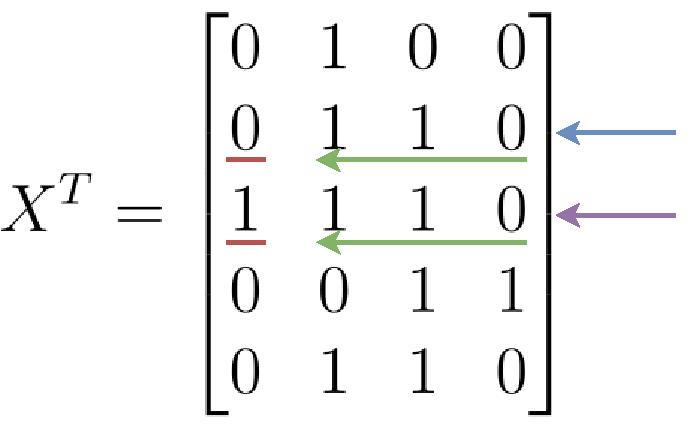
\includegraphics[scale = 0.38]{img/slppanel.pdf}
\end{figure}
Per rendere possibile questa operazione quindi il pannello deve essere sia
salvato come un'unica riga, per ottenerne l'\textit{SLP}, che ``da destra a
sinistra'', per permettere le \textit{LCE query}. Si procede quindi concatenando
ogni riga, selezionandole consecutivamente e leggendone i singoli elementi da
destra a sinistra ottenendo, con colorate gli stessi risultati della query fatta
sopra:
\[0010\,\,{\color{nordgreen}011}{\color{nordred}0}\,\,
  {\color{nordgreen}011}{\color{nordred}1} \,\,1100\,\,0110\]
\textit{Si noti che qui si sono segnalate le varie righe con uno spazio ma solo
  per praticità ``visiva''.}